\thispagestyle{plain}

\section{Números enteros (positivos y negativos)}
Los números positivos son aquellos mayores que cero, como $1, 2, 3, \ldots$. Por otro lado, los números negativos son aquellos menores que cero y están precedidos por el signo menos ($-$), como $-1, -2, -3, \ldots$. Ambos tipos de números se encuentran en la recta numérica:

\begin{center}
    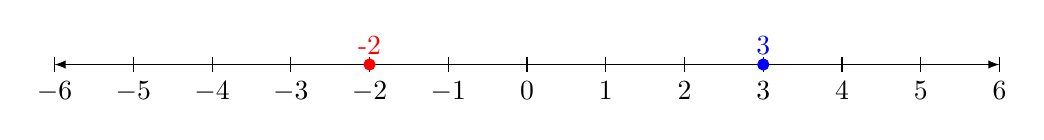
\begin{tikzpicture}
        % Numeric line
        \draw[latex-latex] (-6,0) -- (6,0);
        \foreach \x in {-6,-5,-4,-3,-2,-1,0,1,2,3,4,5,6}
        \draw (\x,0.1) -- (\x,-0.1);
        \foreach \x/\label in {-6/-6,-5/-5,-4/-4,-3/-3,-2/-2,-1/-1,0/0,1/1,2/2,3/3,4/4,5/5,6/6}
        \node[below] at (\x,-0.1) {$\label$};

        % Positive and negative points
        \filldraw[blue] (3,0) circle (2pt) node[above] {3};
        \filldraw[red] (-2,0) circle (2pt) node[above] {-2};
    \end{tikzpicture}
\end{center}

\subsection{Signo de los números enteros}
El signo de un número nos indica si es positivo o negativo. Un número positivo no lleva ningún signo, mientras que un número negativo lleva el signo menos ($-$) delante de él. Por ejemplo, el número 4 es positivo, y el número $-4$ es negativo.

En la recta numérica, un número positivo se ubica a la derecha del cero, mientras que un número negativo se coloca a la izquierda del cero.

\section{Aritmética de números enteros (positivos y negativos)}
En esta sección, aprenderemos cómo sumar y restar números enteros, incluyendo tanto números positivos como negativos. Utilizaremos rectas numéricas para ilustrar los conceptos.

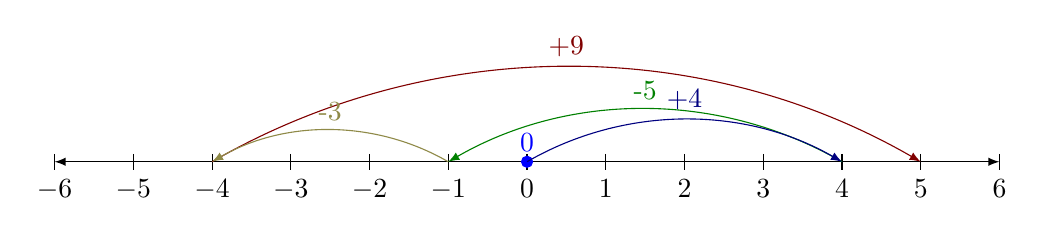
\begin{tikzpicture}
    % Numeric line
    \draw[latex-latex] (-6,0) -- (6,0);
    \foreach \x in {-6,-5,-4,-3,-2,-1,0,1,2,3,4,5,6}
    \draw (\x,0.1) -- (\x,-0.1);
    \foreach \x/\label in {-6/-6,-5/-5,-4/-4,-3/-3,-2/-2,-1/-1,0/0,1/1,2/2,3/3,4/4,5/5,6/6}
    \node[below] at (\x,-0.1) {$\label$};

    % Starting point
    \filldraw[blue] (0,0) circle (2pt) node[above] {0};

    % operations written backwards
    % Adding 9
    \draw[red!50!black,-latex] (-4,0) arc (120:60:9) node[midway,above] {+9};
    % Substract 3
    \draw[yellow!50!black,-latex] (-1,0) arc (60:120:3) node[midway,above] {-3};
    % Substract 5
    \draw[green!50!black,-latex] (4,0) arc (60:120:5) node[midway,above] {-5};
    % Adding 4
    \draw[blue!50!black,-latex] (0,0) arc (120:60:4) node[midway,above] {+4};
\end{tikzpicture}

\subsection{Adición de n\'umeros enteros}
Para sumar dos números enteros, podemos utilizar el concepto de moverse a la derecha en la línea numérica para representar números positivos y a la izquierda para números negativos. Veamos algunos ejemplos:

\subsubsection{Suma de numeros enteros positivos}
Consideremos la suma de $3 + 5$:
\begin{tikzpicture}
    % Numeric line
    \draw[latex-latex] (-1,0) -- (8,0);
    \foreach \x in {-1,0,1,2,3,4,5,6,7,8}
    \draw (\x,0.1) -- (\x,-0.1);
    \foreach \x/\label in {-1/-1,0/0,1/1,2/2,3/3,4/4,5/5,6/6,7/7,8/8}
    \node[below] at (\x,-0.1) {$\label$};

    % Starting point
    \filldraw[blue] (3,0) circle (2pt) node[above] {3};

    % Moving right
    \filldraw[red,-{Latex[length=3mm]}] (3,0) -- (8,0) node[midway,above] {+5};
    \filldraw[blue] (8,0) circle (2pt) node[above] {8};
\end{tikzpicture}

Por lo tanto, $3 + 5 = 8$.

\subsubsection{Suma de numeros enteros positivos y negativos}
Ahora, sumemos $(-2) + 4$:
\begin{tikzpicture}
    % Numeric line
    \draw[latex-latex] (-5,0) -- (6,0);
    \foreach \x in {-5,-4,-3,-2,-1,0,1,2,3,4,5,6}
    \draw (\x,0.1) -- (\x,-0.1);
    \foreach \x/\label in {-5/-5,-4/-4,-3/-3,-2/-2,-1/-1,0/0,1/1,2/2,3/3,4/4,5/5,6/6}
    \node[below] at (\x,-0.1) {$\label$};

    % Starting point
    \filldraw[blue] (-2,0) circle (2pt) node[above] {-2};

    % Moving right
    \filldraw[red,-{Latex[length=3mm]}] (-2,0) -- (2,0) node[midway,above] {+4};
    \filldraw[blue] (2,0) circle (2pt) node[above] {2};
\end{tikzpicture}

Por lo tanto, $(-2) + 4 = 2$.

\subsubsection{Suma de numeros enteros negativos}
Por último, sumemos $(-5) + (-3)$:
\begin{tikzpicture}
    % Numeric line
    \draw[latex-latex] (-8,0) -- (1,0);
    \foreach \x in {-8,-7,-6,-5,-4,-3,-2,-1,0,1}
    \draw (\x,0.1) -- (\x,-0.1);
    \foreach \x/\label in {-8/-8,-7/-7,-6/-6,-5/-5,-4/-4,-3/-3,-2/-2,-1/-1,0/0,1/1}
    \node[below] at (\x,-0.1) {$\label$};

    % Starting point
    \filldraw[blue] (-5,0) circle (2pt) node[above] {-5};

    % Moving left
    \filldraw[red,-{Latex[length=3mm]}] (-5,0) -- (-8,0) node[midway,above] {+(-3)};
    \filldraw[blue] (-8,0) circle (2pt) node[above] {-8};
\end{tikzpicture}

Por lo tanto, $(-5) + (-3) = -8$.

\subsubsection{Conmutatividad aditiva}

\subsection{Resta de n\'umeros enteros}
La resta de números enteros puede pensarse como sumar el opuesto (o inverso aditivo) del número. Veamos algunos ejemplos:

\subsubsection{Resta de numeros enteros positivos}
Consideremos $7 - 3$:
\begin{tikzpicture}
    % Numeric line
    \draw[latex-latex] (2,0) -- (8,0);
    \foreach \x in {2,3,4,5,6,7,8}
    \draw (\x,0.1) -- (\x,-0.1);
    \foreach \x/\label in {2/2,3/3,4/4,5/5,6/6,7/7,8/8}
    \node[below] at (\x,-0.1) {$\label$};

    % Starting point
    \filldraw[blue] (7,0) circle (2pt) node[above] {7};

    % Moving left
    \filldraw[red,-{Latex[length=3mm]}] (7,0) -- (2,0) node[midway,above] {+(-3)};
    \filldraw[blue] (2,0) circle (2pt) node[above] {4};
\end{tikzpicture}

Por lo tanto, $7 - 3 = 4$.

\subsubsection{Resta de numeros enteros negativos}
Ahora, restemos $5 - (-2)$:
\begin{tikzpicture}
    % Numeric line
    \draw[latex-latex] (-3,0) -- (6,0);
    \foreach \x in {-3,-2,-1,0,1,2,3,4,5,6}
    \draw (\x,0.1) -- (\x,-0.1);
    \foreach \x/\label in {-3/-3,-2/-2,-1/-1,0/0,1/1,2/2,3/3,4/4,5/5,6/6}
    \node[below] at (\x,-0.1) {$\label$};

    % Starting point
    \filldraw[blue] (5,0) circle (2pt) node[above] {5};

    % Moving right
    \filldraw[red,-{Latex[length=3mm]}] (5,0) -- (0,0) node[midway,above] {+2};
    \filldraw[blue] (0,0) circle (2pt) node[above] {2};
\end{tikzpicture}

Por lo tanto, $5 - (-2) = 7$.
\subsubsection{Resta de  dos numeros negativos}
Por último, restemos $(-4) - (-7)$:
\begin{tikzpicture}
    % Numeric line
    \draw[latex-latex] (-8,0) -- (1,0);
    \foreach \x in {-8,-7,-6,-5,-4,-3,-2,-1,0,1}
    \draw (\x,0.1) -- (\x,-0.1);
    \foreach \x/\label in {-8/-8,-7/-7,-6/-6,-5/-5,-4/-4,-3/-3,-2/-2,-1/-1,0/0,1/1}
    \node[below] at (\x,-0.1) {$\label$};

    % Starting point
    \filldraw[blue] (-4,0) circle (2pt) node[above] {-4};

    % Moving right
    \filldraw[red,-{Latex[length=3mm]}] (-4,0) -- (0,0) node[midway,above] {+7};
    \filldraw[blue] (0,0) circle (2pt) node[above] {3};
\end{tikzpicture}

Por lo tanto, $(-4) - (-7) = 3$.
\newpage